\subsection{Scenario 3: Unauthorized State Change and Data Exfiltration}

\subsubsection{Introduction and Objectives}
Scenario 3 advances the adversarial narrative estblished in the previous scenario from initial network compromise to post-exploitation, focusing specifically on data exfiltration and stealthy Command and Control (C2) communication. In this phase, the previously compromised Smart Camera is manipulated by the internal attacker node (\texttt{10.0.0.3}) to completely bypass its authorized constraints. To capture this dynamic, a new external adversarial (\texttt{203.0.113.5}) is introduced to act as the destination for the stolen data. The primary objective is to measure and document how post-exploitation routing anomalies and application-layer manipulations deviate from the Scenario 1 control baseline. The scenario goals in detail are the following:

\begin{enumerate}
	\item Execute a targeted trigger payload from the internal attacker to the Smart Camera's TLS control channel at a precise temporal marker ($t=300$ seconds). This simulates the localized activation of malware or a malicious configuration update, initiating the exfiltration sequence without generating broad network noise.
	\item Demonstrate rogue data exfiltration and port masquerading. The Smart Camera will be forced to terminate its authorized local video stream and redirect the high-bandwidth UDP payload directly to the external rogue IP address. This exfiltration stream is deliberately mapped to port 443 to masquerade as benign outbound HTTPS traffic, challenging basic port-based firewall heuristics.
	\item Execute a stealthy DNS hijacking maneuver. The compromised camera will seamlessly shift its domain name resolution requests to a malicious C2 domain (e.g., \texttt{c2.malicious-exfil.com}) while strictly maintaining its baseline 60-second polling frequency. This demonstrates an advanced evasion tactic designed to bypass purely volumetric anomaly detection by preserving statistical temporal normality.
\end{enumerate}


\subsubsection{Expected Behaviour and Theoretical Baselines}

To ensure statistical significance and provide a robust dataset for comparative feature extraction, Scenario 3 has similarly been executed over a 1200-second (20-minute) capture period. 

Unlike the highly visible, noisy volumetric attacks observed in Scenario 2, this scenario expects to demonstrate stealthy, post-exploitation behavior. The anticipated forensic deviations from the control baseline are:

\begin{itemize}
	\item \textbf{Volumetric Camouflage (Flow Density Deception):} Unlike the massive flow spikes caused by the prior network scan and brute-force attacks, Scenario 3 is engineered to evade basic volumetric anomaly detection. Because the attacker only sends a single trigger payload at $t=300$, and the compromised camera simply redirects its existing bandwidth rather than creating new noise, the aggregate network flow density (flows per minute) is expected to falsely appear as a stable, healthy baseline. The main difference will be that the flow will be directed to a different port and domain. 
	
	\item \textbf{Protocol Masquerading (Port Inversion):} Following the payload trigger, the camera will terminate its authorized local video stream (UDP port 50005) and initiate a new data exfiltration stream. To bypass egress firewall filtering, this massive volumetric stream will target port 443. This will severely corrupt the network's protocol-to-port expectations, logging an anomalous, high-bandwidth UDP stream operating over a port traditionally reserved for TCP-based TLS traffic.
	
	\item \textbf{Evasive Application-Layer Manipulation (DNS Hijacking):} The compromised camera will maintain its mathematically rigid 60 seconds Inter-Arrival Time (IAT) for DNS queries, further masking the attack from temporal flow analysis. However, it is expected to resolve a total different domain name, the C2 one in this case.
	
	\item \textbf{External Adjacency Matrix Violation (MUD Corruption):} The Topology Interaction Heatmap will log a cessation of the camera's heavy video traffic to the Gateway, instantly replaced by a massive new density cluster directed toward the unauthorized rogue cloud IP (\texttt{203.0.113.5}). This provides absolute visual proof of a critical Manufacturer Usage Description (MUD) profile breach.
\end{itemize}

\subsubsection{Evidence Integrity and Feature Extraction}
The same steps of \ref{evidence_integrity} have been followed to guarantee the integrity and validity of the extracted features. 

\paragraph{MUD Profile Validation}\mbox{}\\

The first step is to compare again the expected baseline behaviour to the observed empirical results with the objectivo to detect attacker activity. 

\begin{table}[H]
	\centering
	\renewcommand{\arraystretch}{1.2}
	% Resizebox forces the table to perfectly fit the text width of your page
	\resizebox{\textwidth}{!}{%
		\begin{tabular}{@{}l c c l@{}}
			\toprule
			\textbf{Traffic Classification Profile} & \textbf{Expected} & \textbf{Empirical} & \textbf{Status / Delta} \\ 
			\midrule
			\multicolumn{4}{@{}l}{\textbf{Authorized IoT Services}} \\
			NTP Synchronization (UDP/123) & 6 & 6 & $\checkmark$ Baseline Match \\
			MQTT Keep-Alives (TCP/8883) & 121 & 121 & $\checkmark$ Baseline Match \\
			MQTT Telemetry Payloads (TCP/8883) & 5 & 5 & $\checkmark$ Baseline Match \\
			Video Feed Stream (to Gateway/50005) & 1 & 1 & $\checkmark$ Terminated Early \\
			TLS Cloud Telemetry (TCP/443) & 5 & 5 & $\checkmark$ Baseline Match \\
			\addlinespace
			\multicolumn{4}{@{}l}{\textbf{Adversarial \& Post-Exploitation Activity}} \\
			DNS Queries (UDP/53) & 42 & 57 & $\times$ Hijacked C2 Polling (+15) \\
			Attacker Trigger Payload (TCP/443) & 0 & 1 & $\times$ Compromise Event \\
			UDP Data Exfiltration (to Rogue/443) & 0 & 1 & $\times$ Egress MUD Violation \\
			Zeek QUIC Protocol Anomalies & 0 & 1 & $\times$ Masquerading Detected \\
			\addlinespace
			\multicolumn{4}{@{}l}{\textbf{Environmental Noise / Infrastructure}} \\
			Background ICMP \& Packet Filter Notes & 0 & 2 & $\sim$ Minor Hypervisor Noise \\
			\midrule
			\textbf{Total Connection Flows} & \textbf{180} & \textbf{199} & \textbf{Stealth Profile (+10.5\%)} \\
			\bottomrule
		\end{tabular}%
	}
	\caption{Scenario 3: Comparative Traffic Breakdown (Stealth Exfiltration \& C2 Routing)}
	\label{tab:scenario3_traffic}
\end{table}

\textbf{As expected, attacker activity has been registered, though characterized by extreme stealth.} In contrast to the 3,459\% spike observed in Scenario 2, the data exfiltration attack generated only a 10.5\% volumetric increase (199 total connections). Because the attacker utilized a single TCP trigger payload and maintained the camera's baseline DNS polling frequency, the aggregate network density failed to trigger standard volumetric thresholds. 

This minimal structural deviation proves that while legitimate device operations continue, sophisticated post-exploitation tactics can seamlessly blend into the authorized traffic baseline. This provides possible justification for application aware security engines: without analyzing the deep packet metadata (such as port 443 protocol masquerading and DNS domain anomalies), the exfiltration stream can remain functionally invisible to traditional network monitors.

\paragraph{Camera Behaviour: Exfiltration \& Port Masquerading}\mbox{}\\
The observed transmission behavior of the Smart Camera (Figure \ref{fig:camera_exfil}) highlights the critical danger of post-exploitation data exfiltration. At a macro volumetric level, the camera's total outbound throughput does not change, avoiding the asymmetric throughput anomalies that trigger basic firewalls. 

Instead, the anomaly is entirely topological. The graph clearly highlights the operational shift at $t=300$ (05:00). Following the attacker's trigger, the camera completely ceases its authorized UDP transmission to the local Gateway on port 50005. Immediately, an equivalent volume of high-density UDP traffic is spun up and redirected to the external rogue cloud infrastructure. By pushing this exfiltration stream through port 443, the attacker successfully camouflages the hijacked video feed, violating the device's zero-trust MUD profile without alerting pure bandwidth-threshold monitors.

\paragraph{DNS Resolution and C2 Polling}\mbox{}\\
In addition to the port masquerading, the attack successfully altered the device's domain name resolution behavior. The empirical data recorded a total of 57 DNS queries, exceeding the zero-trust baseline expectation by 15 requests. 

This numerical deviation maps precisely to the attack timeline. Following the compromise at the 5-minute mark, the camera began resolving an unauthorized Command and Control (C2) domain alongside its standard operations. By executing these malicious queries at a steady 60-second interval over the remaining 15 minutes of the capture, the attacker generated exactly 15 anomalous DNS requests. This can highlight a possible vulnerability since without application-layer visibility into the specific queried domains, the device's lateral connection to the adversarial infrastructure remains entirely hidden.

\paragraph{Thermostat Behaviour}\mbox{}\\
The Smart Thermostat sees no changes in behaviour since it is not the target of the attack.

\paragraph{Other Metrics}\mbox{}\\

As illustrated in Figure \ref{fig:networkflowdensity}, the empirical flow density exhibits three distinct volumetric anomalies. Rather than a random distribution of noise, these deviations perfectly map to the chronological execution of the adversarial kill chain:

\begin{itemize}
	\item \textbf{Phase 1: The Reconnaissance Surge (Initial Spike):} The massive, immediate vertical spike observed at the beginning of the timeline represents the automated subnet and port sweep. Because network scanners operate asynchronously—flooding the target with thousands of simultaneous \texttt{SYN} probes to enumerate open ports—this phase generates an explosive but brief density maximum before the scanner concludes its mapping phase.
	
	\item \textbf{Phase 2: The Brute-Force Plateau (Sustained Volatility):} Following the initial scan, the graph does not return to the authorized baseline of $\sim$8 flows per minute. Instead, it transitions into a sustained plateau. This elevated constant peak represents the credential brute-force attack against the Smart Camera's TLS control channel (TCP port 443). The script executes rapid, iterative login attempts, generating a persistent high-density noise floor that persists for the majority of the attack window.
	
	\item \textbf{Phase 3: The Payload Injection (Terminal Anomaly):} Near the conclusion of the capture window, the brute-force plateau ceases, followed by a final, microscopic spike of exactly 12 flows. Forensically, this is the most critical metric on the timeline: it represents the moment of successful authentication and the subsequent injection of the malicious configuration payload, effectively altering the edge device's operational state just before the attacker terminates the session.
\end{itemize}

\begin{figure}[H]
	\centering
	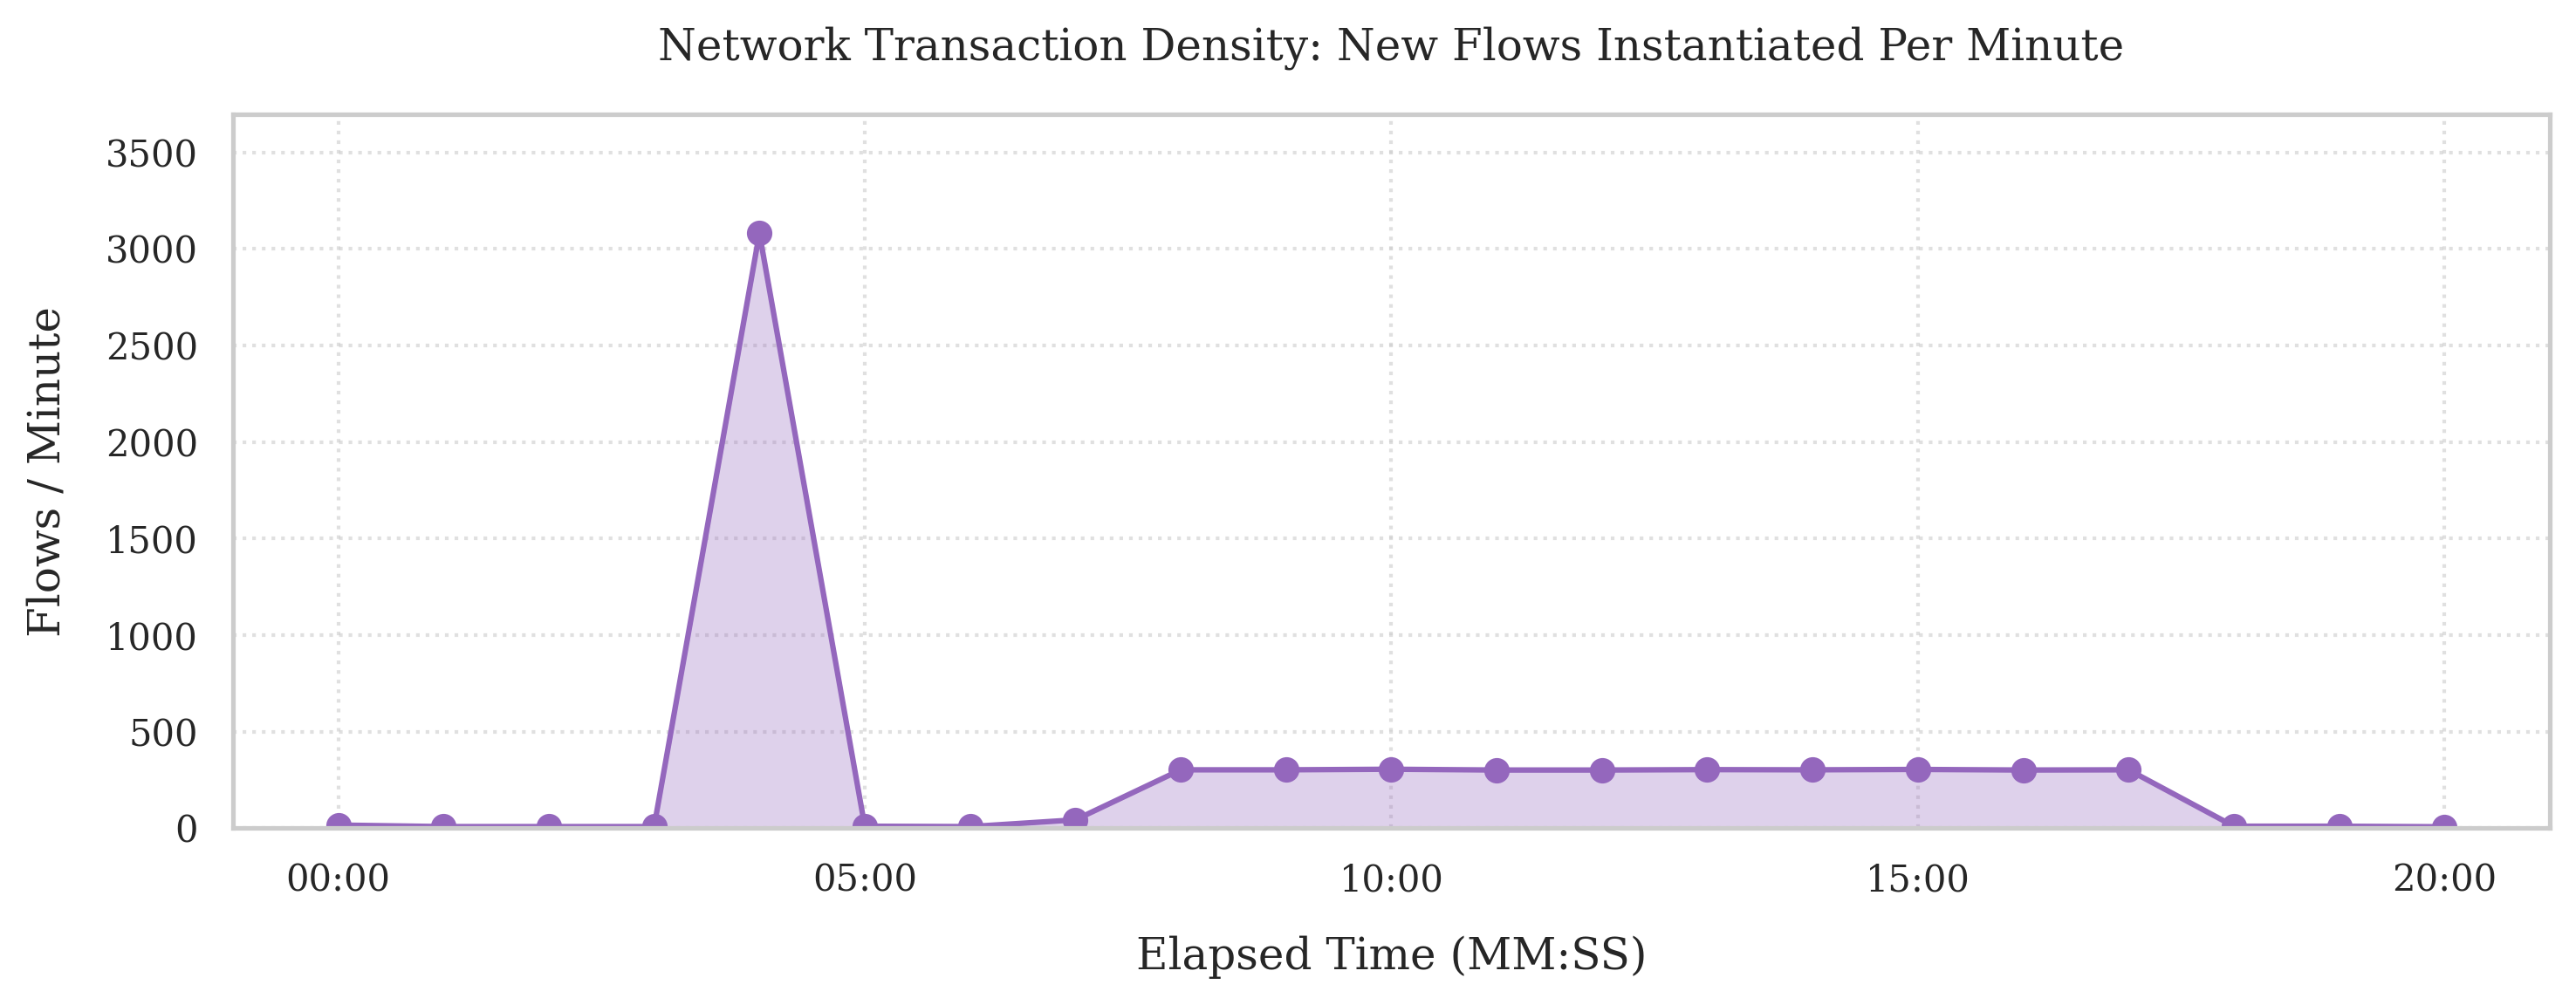
\includegraphics[width=0.9\linewidth]{../figures/scenario2/network_flow_density}
	\caption{Network Flow Density (Scenario2).}
	\label{fig:networkflowdensity}
\end{figure}

The TCP connection state distribution, also provides clear structural proof of the attack's impact on the network. As seen in Scenario 1, In a stable baseline, TCP flows primarily resolve with an \texttt{SF} (Normal) state flag, indicating successful connections and clean teardowns. While authorized IoT traffic continued normally during the attack (registering 133 \texttt{SF} flows), it was completely eclipsed by a massive surge in anomalous activity. 

Specifically, Zeek recorded 6,041 flows terminating in a \texttt{REJ} (Rejected) state. This flag is logged when a target actively refuses a connection attempt via a TCP Reset (RST) packet. This spike in rejected handshakes is the direct footprint of the attacker (\texttt{10.0.0.3}) scanning the network. As the scanner flooded the IoT edge devices with \texttt{SYN} probes targeting closed ports, the devices continuously issued RST packets to block the unauthorized access. 

Consequently, this sudden inversion of the \texttt{SF}-to-\texttt{REJ} ratio serves as an ideal, automated tripwire for detecting an active internal breach.

\begin{figure}[H]
	\centering
	
\includegraphics[width=0.9\linewidth]{../../iot_forensics_project/figures/scenario2/tcp_connection_states}
	\caption{TCP Connection State Distribution (Scenario 2).}
	\label{fig:tcpconnectionstates}
\end{figure}

Finally, the interaction heatmaps is totally altered, in this scenario is exposing a network heavily saturated with unauthorized cross-node communications. The baseline has been broken by the attacker node which acts as the origin for all anomalous traffic. The matrix clearly distinguishes the broad network reconnaissance, evidenced by the 1,025 probes sent to both the Gateway and the Thermostat, from the targeted exploitation of the Smart Camera, which absorbed 3996 direct connections.


\begin{figure}[H]
	\centering
	
\includegraphics[width=0.9\linewidth]{../../iot_forensics_project/figures/scenario2/topology_traffic_matrix}
	\caption{Empirical interaction heatmap detailing authorized internal network flows (Scenario 2).}
	\label{fig:topologytrafficmatrix}
\end{figure}


